%%%%%%%%%%%%%%%%%%%%%%%%%%%%%%%%%%%%%%%%%
% University Assignment Title Page 
% LaTeX Template
% Version 1.0 (27/12/12)
%
% This template has been downloaded from:
% http://www.LaTeXTemplates.com
%
% Original author:
% WikiBooks (http://en.wikibooks.org/wiki/LaTeX/Title_Creation)
%
% License:
% CC BY-NC-SA 3.0 (http://creativecommons.org/licenses/by-nc-sa/3.0/)
%
%%%%%%%%%%%%%%%%%%%%%%%%%%%%%%%%%%%%%%%%%
%\title{Title page with logo}
%----------------------------------------------------------------------------------------
%	PACKAGES AND OTHER DOCUMENT CONFIGURATIONS
%----------------------------------------------------------------------------------------

\documentclass[12pt]{article}
\usepackage[english]{babel}
\usepackage[utf8x]{inputenc}
\usepackage{natbib}
\usepackage{amsmath}
\usepackage[colorinlistoftodos]{todonotes}
\usepackage{listings}
\usepackage{color}
\usepackage[explicit]{titlesec}
\usepackage{url}
\usepackage{subfig}
\usepackage{graphicx}
\usepackage{grffile}
\usepackage{tabularx, ragged2e}
\usepackage{diagbox}
\usepackage{float}

\renewcommand\tabularxcolumn[1]{>{\Centering}p{#1}}

\makeatletter
\@addtoreset{section}{part}
\def\@part[#1]#2{%
    \ifnum \c@secnumdepth >\m@ne
      \refstepcounter{part}%
      \addcontentsline{toc}{part}{\thepart\hspace{1em}#1}%
    \else
      \addcontentsline{toc}{part}{#1}%
    \fi
    {\parindent \z@ \raggedright
     \interlinepenalty \@M
     \normalfont\centering
     \ifnum \c@secnumdepth >\m@ne
       \LARGE\bfseries \partname\nobreakspace\thepart
       \par\nobreak
     \fi
     \huge \bfseries #2%
     \markboth{}{}\par}%
    \nobreak
    \vskip 3ex
    \@afterheading}
\renewcommand\partname{Topic}
\makeatother


\definecolor{dkgreen}{rgb}{0,0.6,0}
\definecolor{gray}{rgb}{0.5,0.5,0.5}
\definecolor{mauve}{rgb}{0.58,0,0.82}

\begin{document}

\begin{titlepage}

\newcommand{\HRule}{\rule{\linewidth}{0.5mm}} % Defines a new command for the horizontal lines, change thickness here

\center % Center everything on the page
 
%----------------------------------------------------------------------------------------
%	HEADING SECTIONS
%----------------------------------------------------------------------------------------

\textsc{\LARGE University of St Andrews}\\[1.5cm] % Name of your university/college
\textsc{\Large CS4203 Coursework 2}\\[0.5cm] % Major heading such as course name
\textsc{\large }\\[0.5cm] % Minor heading such as course title

%----------------------------------------------------------------------------------------
%	TITLE SECTION
%----------------------------------------------------------------------------------------

\HRule \\[0.4cm]
{ \huge \bfseries Security Tools}\\[0.4cm] % Title of your document
\HRule \\[1.5cm]
 
%----------------------------------------------------------------------------------------
%	AUTHOR SECTION
%----------------------------------------------------------------------------------------


\Large \emph{Author:}\\
 \textsc{150008022}\\[3cm] % Your name

%----------------------------------------------------------------------------------------
%	DATE SECTION
%----------------------------------------------------------------------------------------

{\large \today}\\[2cm] % Date, change the \today to a set date if you want to be precise

%----------------------------------------------------------------------------------------
%	LOGO SECTION
%---------------------------------------------------------------------------------------


\includegraphics[width = 3.1cm]{images/standrewslogo.png}
 
%----------------------------------------------------------------------------------------

\vfill % Fill the rest of the page with whitespace

\end{titlepage}

\begin{center}
Part I: 1377 Words,
Part II: 1007 Words,
\end{center}


\part*{Goal}

The goal of this practical was to use and evaluate common tools and techniques used in security: steganography and penetration testing.



\part{Steganography}

Least Significant Bit (LSB) steganography - specifically LSB1 - involves replacing the last bit of each byte of an image file (called the cover image) with a bit from the data to be hidden. For example, if each character in the message requires a single byte, then it can be hidden in 8 bytes of the cover image. If we instead use the two least significant bits, we can half the image size needed to mask our message, but this can result in more obvious distortion in the original image. The message being hidden doesn't necessarily have to be text either, images can be masked using other images as well.

Experiment \ref{comparingimages} compares various images after LSB steganography is applied to determine the effectiveness of spatial frequency as a metric for choosing cover images. In experiment \ref{psnrmetric}, the effectiveness of peak signal-to-noise ratio (PSNR) as a metric is also evaluated.

\section{Spatial Frequencies} \label{comparingimages}

\subsection{Introduction}
Images can contain a range of spatial frequencies. High frequency images show fine details, whilst low frequency images consist of smoother transitions between dark and light (See figure \ref{fig:spacefreq}). In this experiment, the effect of LSB on images of varying spatial frequencies is compared, using an online image steganography tool \cite{imagesteg}.

\begin{figure}[htb]
    \centering
    \subfloat[High spatial frequency image]{{\includegraphics[width=5cm]{"images/lsbrgb/face_high_SF"} }}%
    \qquad
    \subfloat[Low spatial frequency image]{{\includegraphics[width=5cm]{"images/lsbrgb/face_low_SF"} }}%
    \caption{Comparison of spatial frequencies in images \cite{spatialfreq}}%
    \label{fig:spacefreq}%
\end{figure}

\subsection{Aims}

The aims of this experiment are:
\begin{enumerate}
	\item to determine if spatial frequency is useful as a metric for choosing an effective cover/hidden image combination. \label{spatialeffectivenessaim}
	\item  to determine whether a high, medium, or low frequency image is a better candidate for a cover file.  \label{stegaimcover}
	\item  to determine which combination of high or low frequency cover image and high or low frequency hidden image provides the best concealment. \label{stegaimhidden}
\end{enumerate}

\subsection{Methods}
In order to reduce the number of variables in this experiment and simplify masking one image in another, the images used were all cropped and scaled to the size of $640\times396$ pixels. Three images were used that contained either low, medium or high values spatial frequency components. The images were viewed on a 15.6" Matte FHD LED IPS display with a resolution of $1920 \times 1080$. The \textit{Eye of GNOME} application was used to open and display the image files
	 
	 A Matlab\textsuperscript{\textregistered} script was written (\textit{showDCT.m}) that converted the images to grayscale and used Discrete Cosine Transform to show the distribution of spatial frequencies. The images used and their spatial frequencies are shown in figures \ref{fig:highfreq} to \ref{fig:highfreq2}. The DCT plots show the lowest frequencies in the top left and the highest frequencies in the bottom right. 

      \begin{figure}[H]
        \center{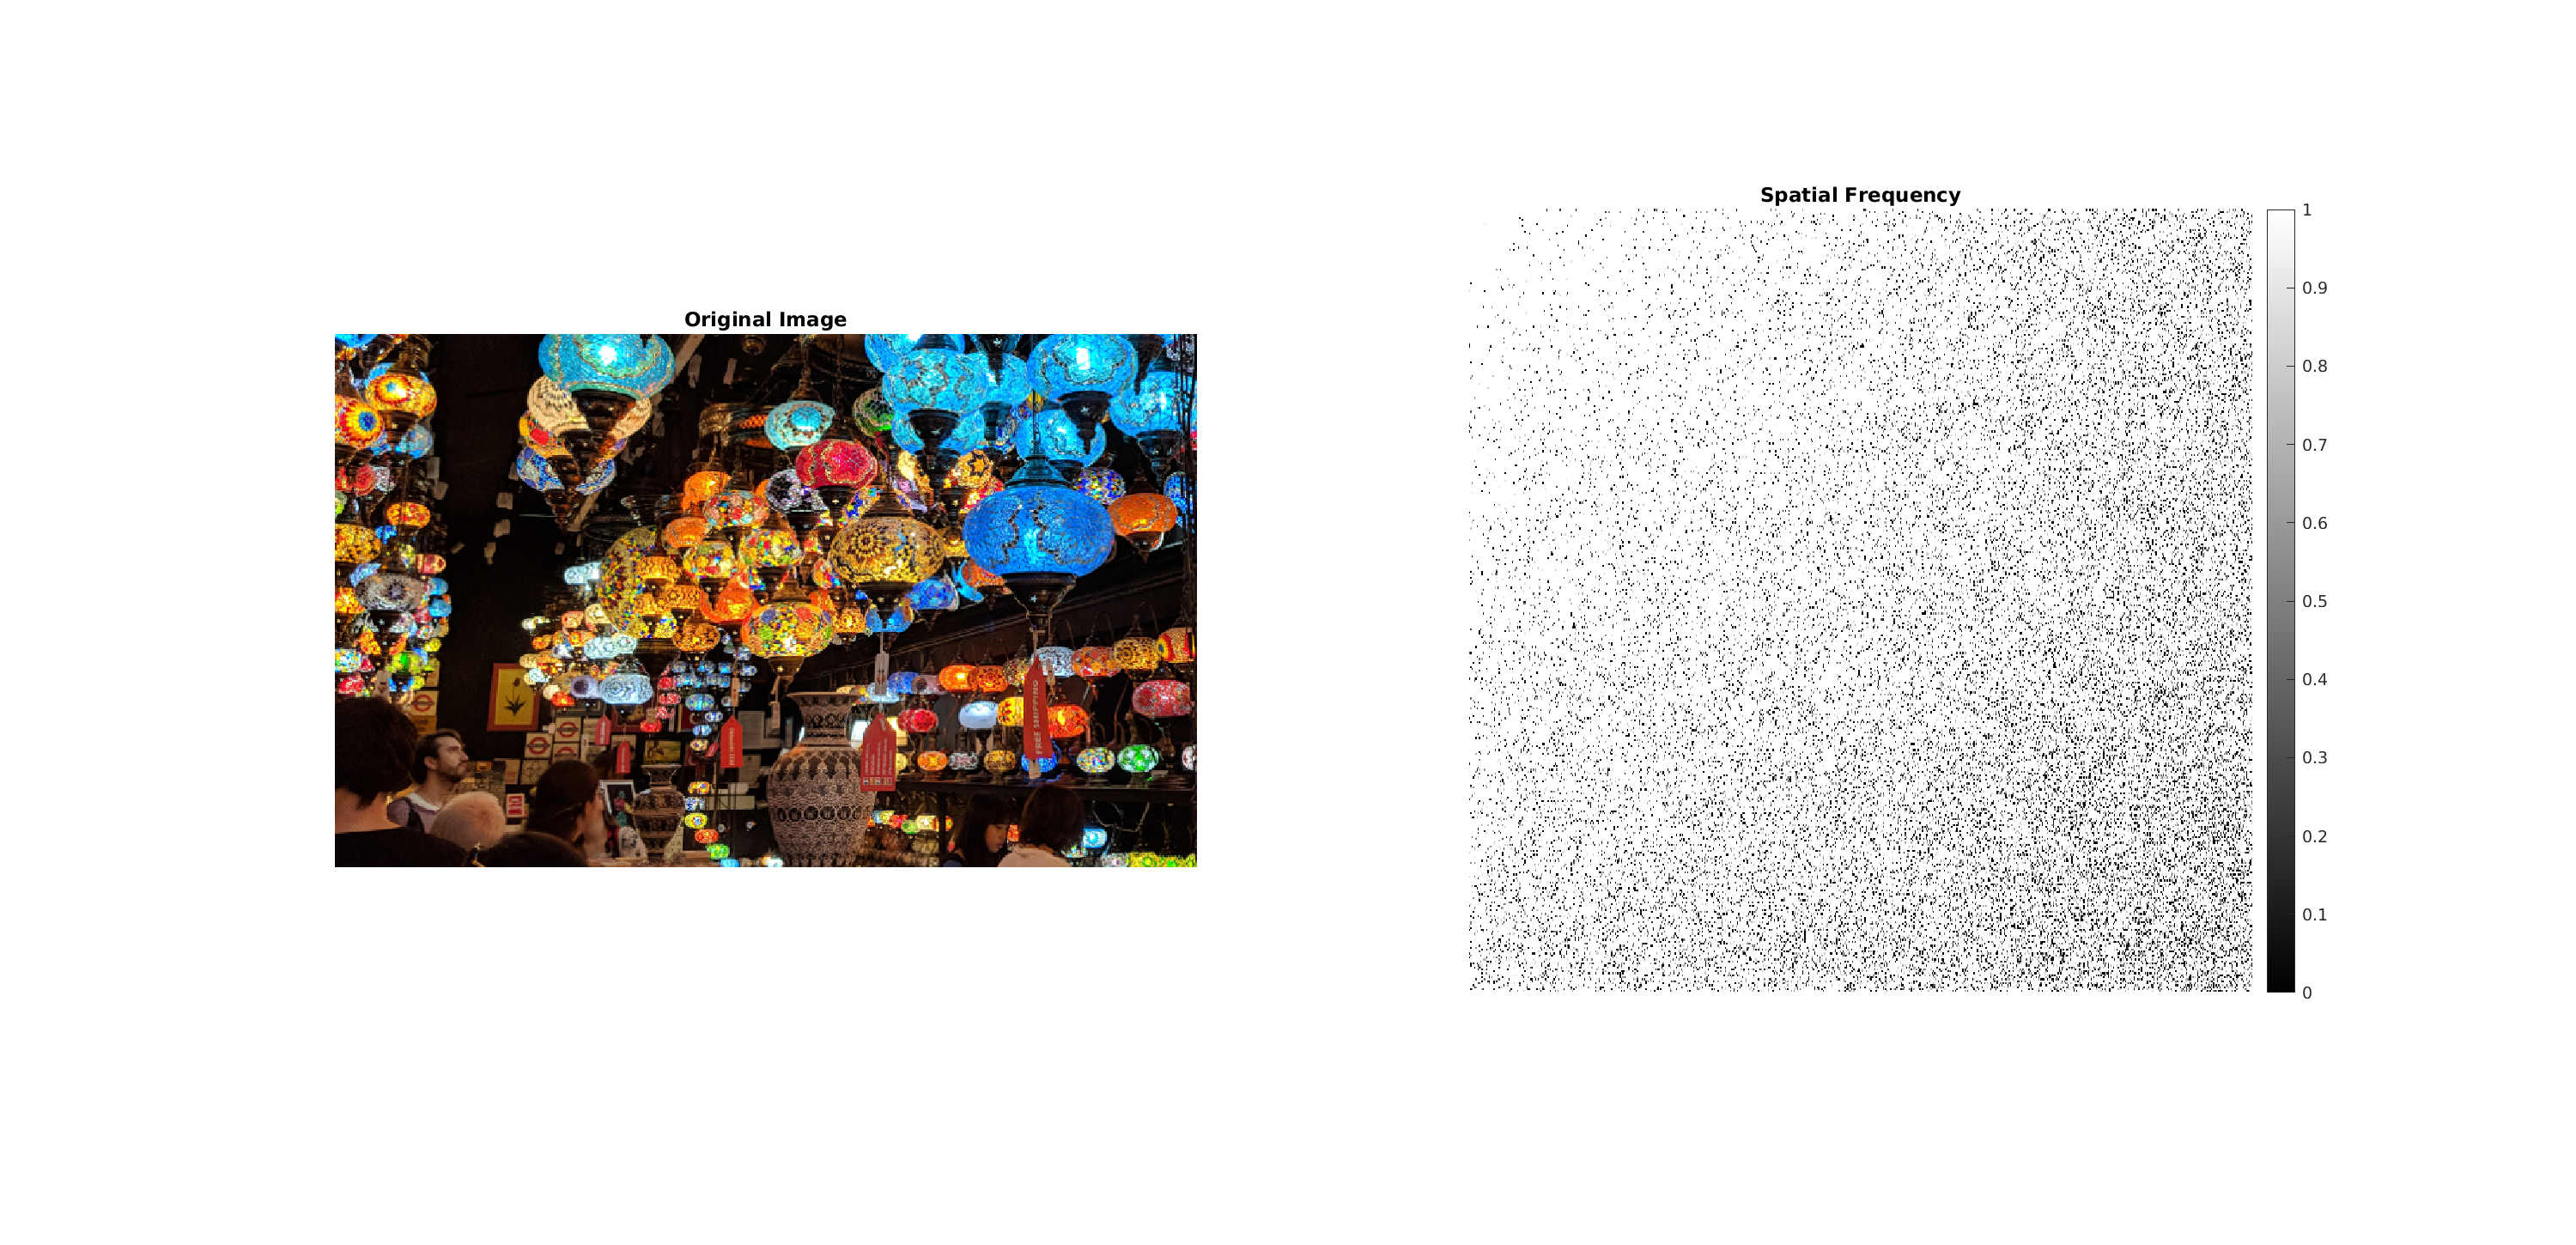
\includegraphics[width=\textwidth]
        {images/lsbrgb/dct/colourful_highfreq_dct.png}}
        \caption{\label{fig:highfreq} "Colourful": High frequency image (left) and spatial frequency distribution (right).}
      \end{figure}
      \begin{figure}[H]
        \center{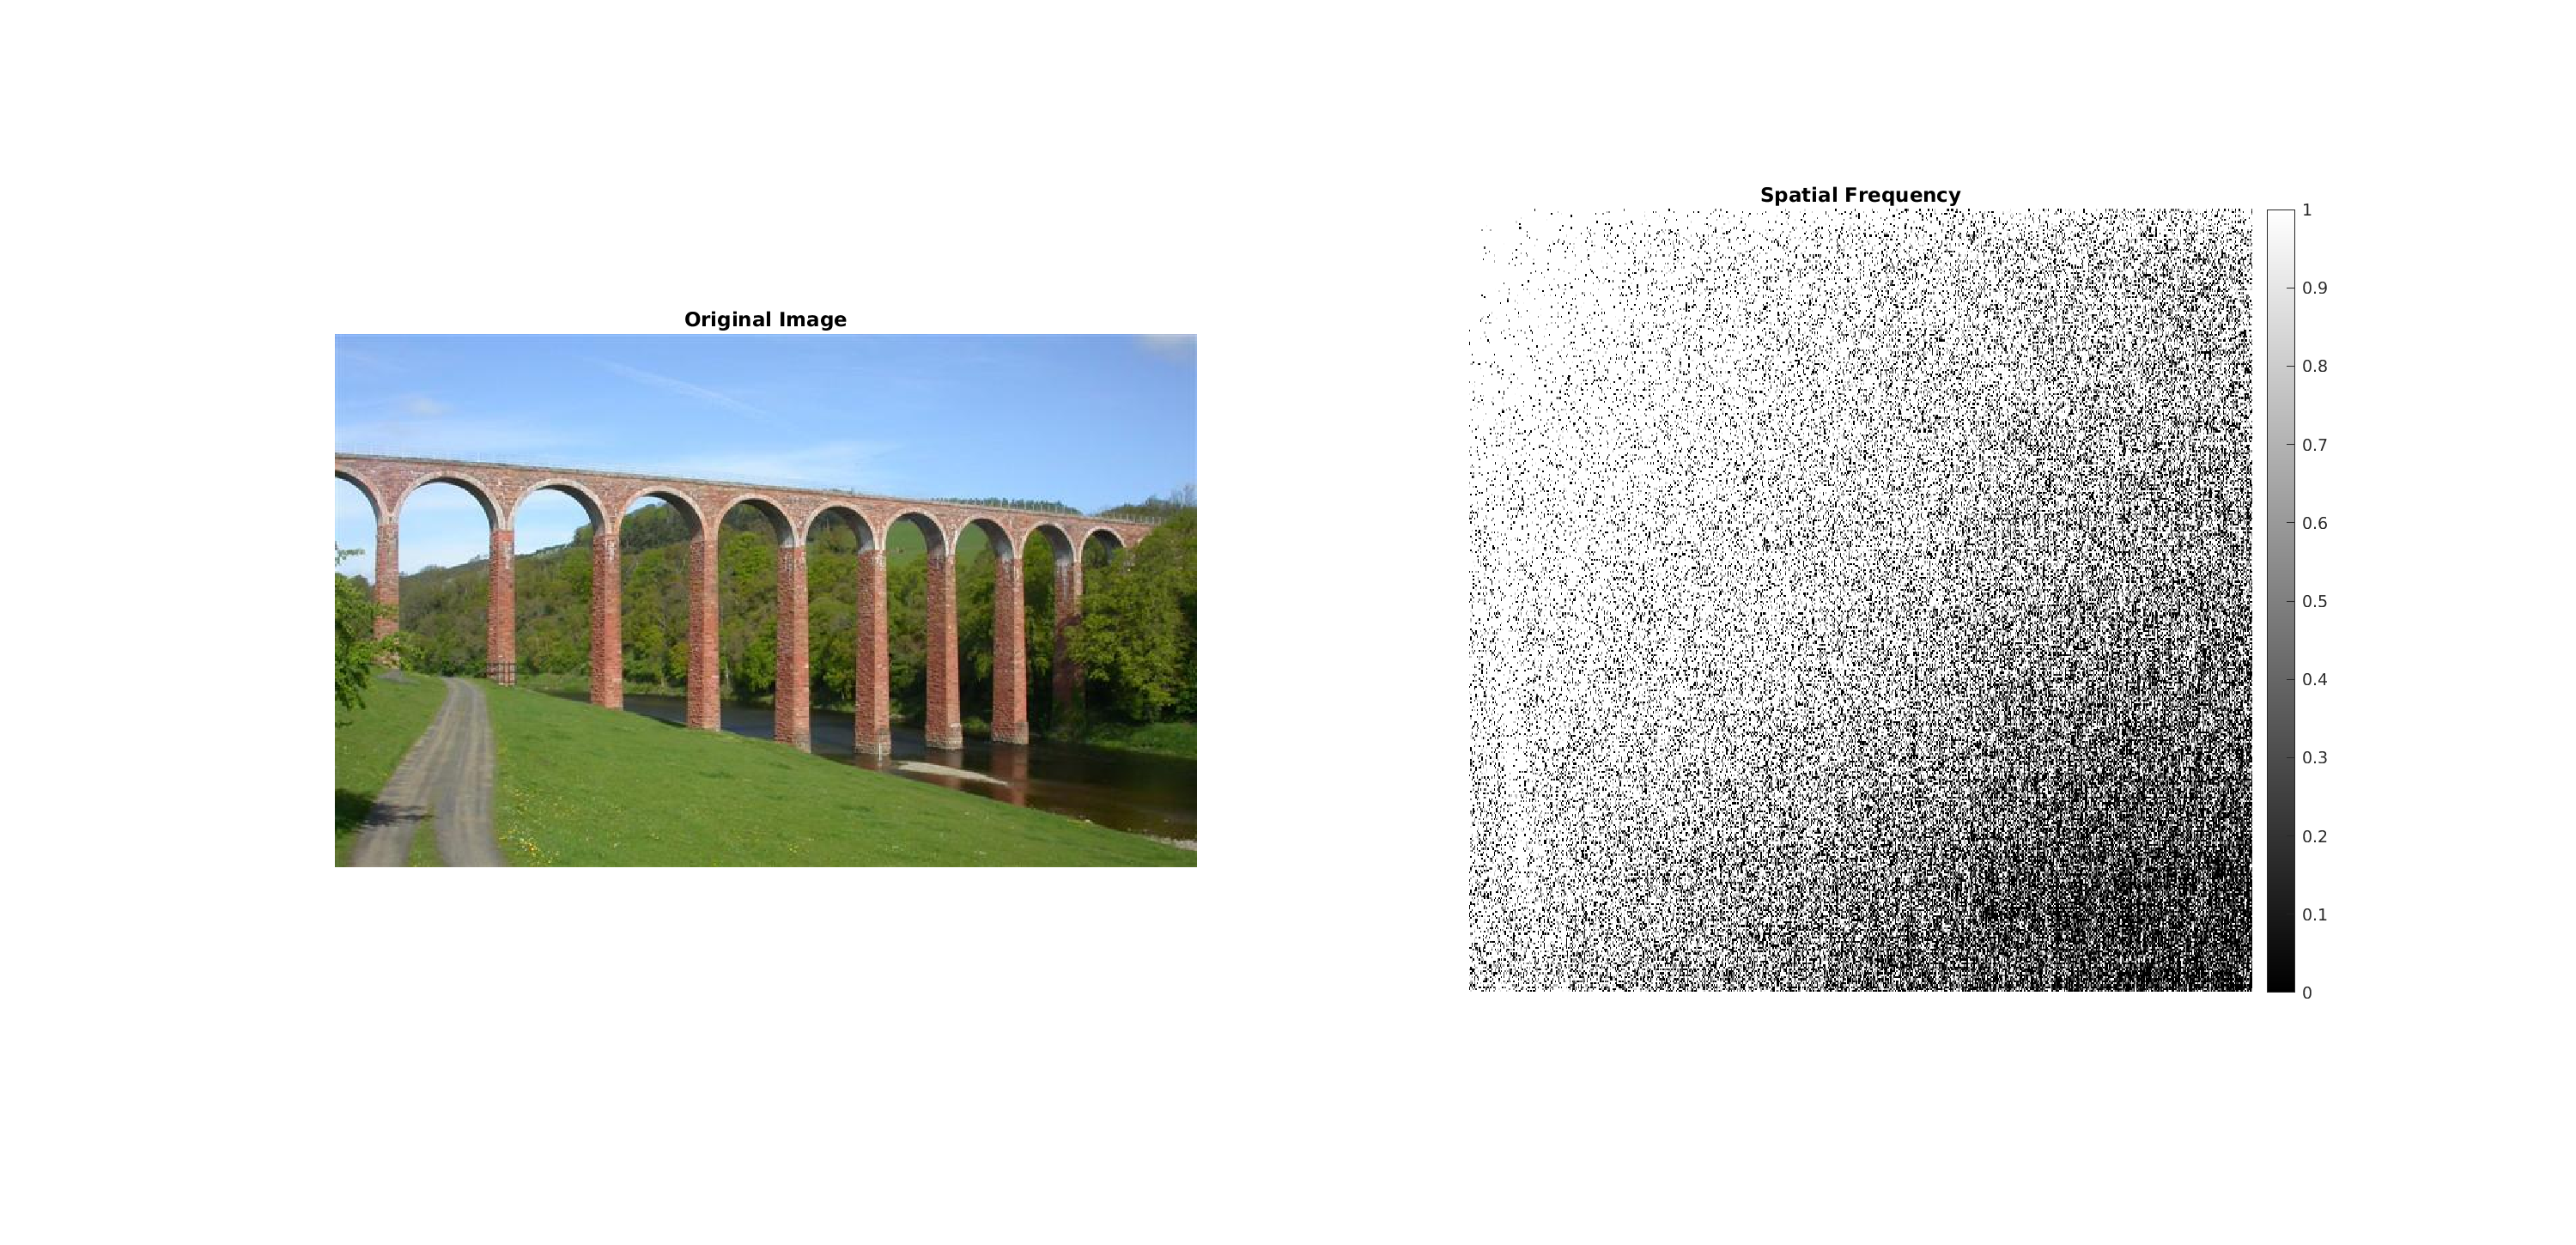
\includegraphics[width=\textwidth]
        {images/lsbrgb/dct/viaduct_medreq_dct.png}}
        \caption{\label{fig:midfreq} "Viaduct": Mid frequency image (left) and spatial frequency distribution (right).}
      \end{figure}
      \begin{figure}[H]
        \center{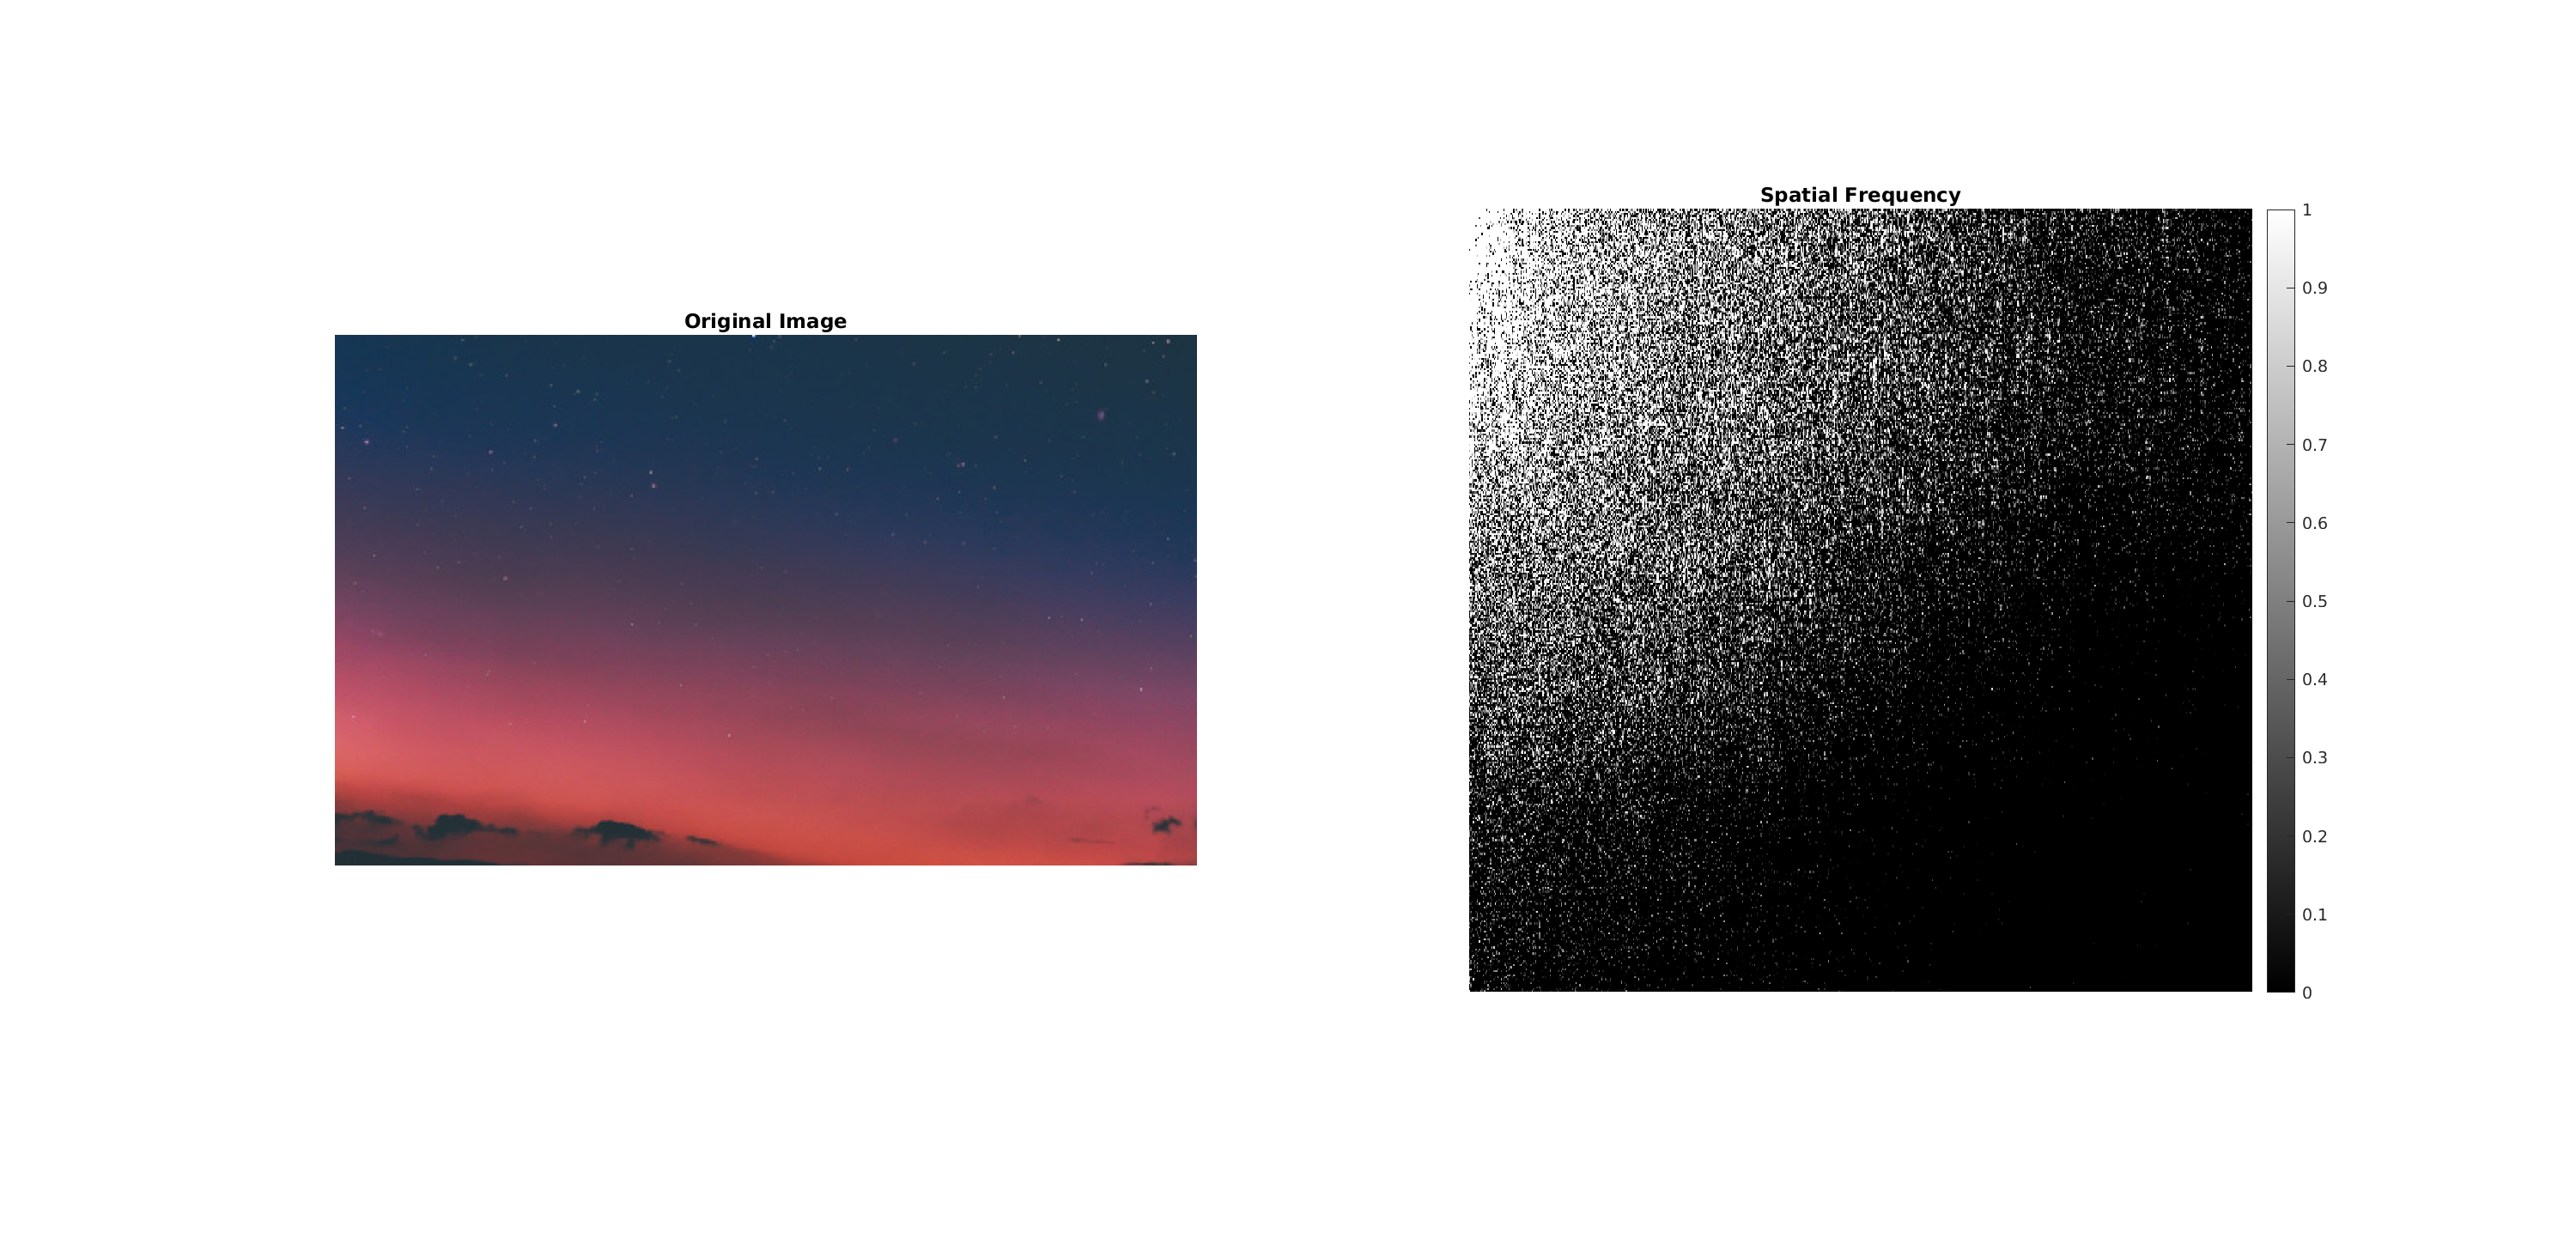
\includegraphics[width=\textwidth]
        {images/lsbrgb/dct/sky_lowfreq_dct.png}}
        \caption{\label{fig:lowfreq} "Sky": Low frequency image \cite{sky} (left) and spatial frequency distribution (right)}.
      \end{figure}
      \begin{figure}[H]
        \center{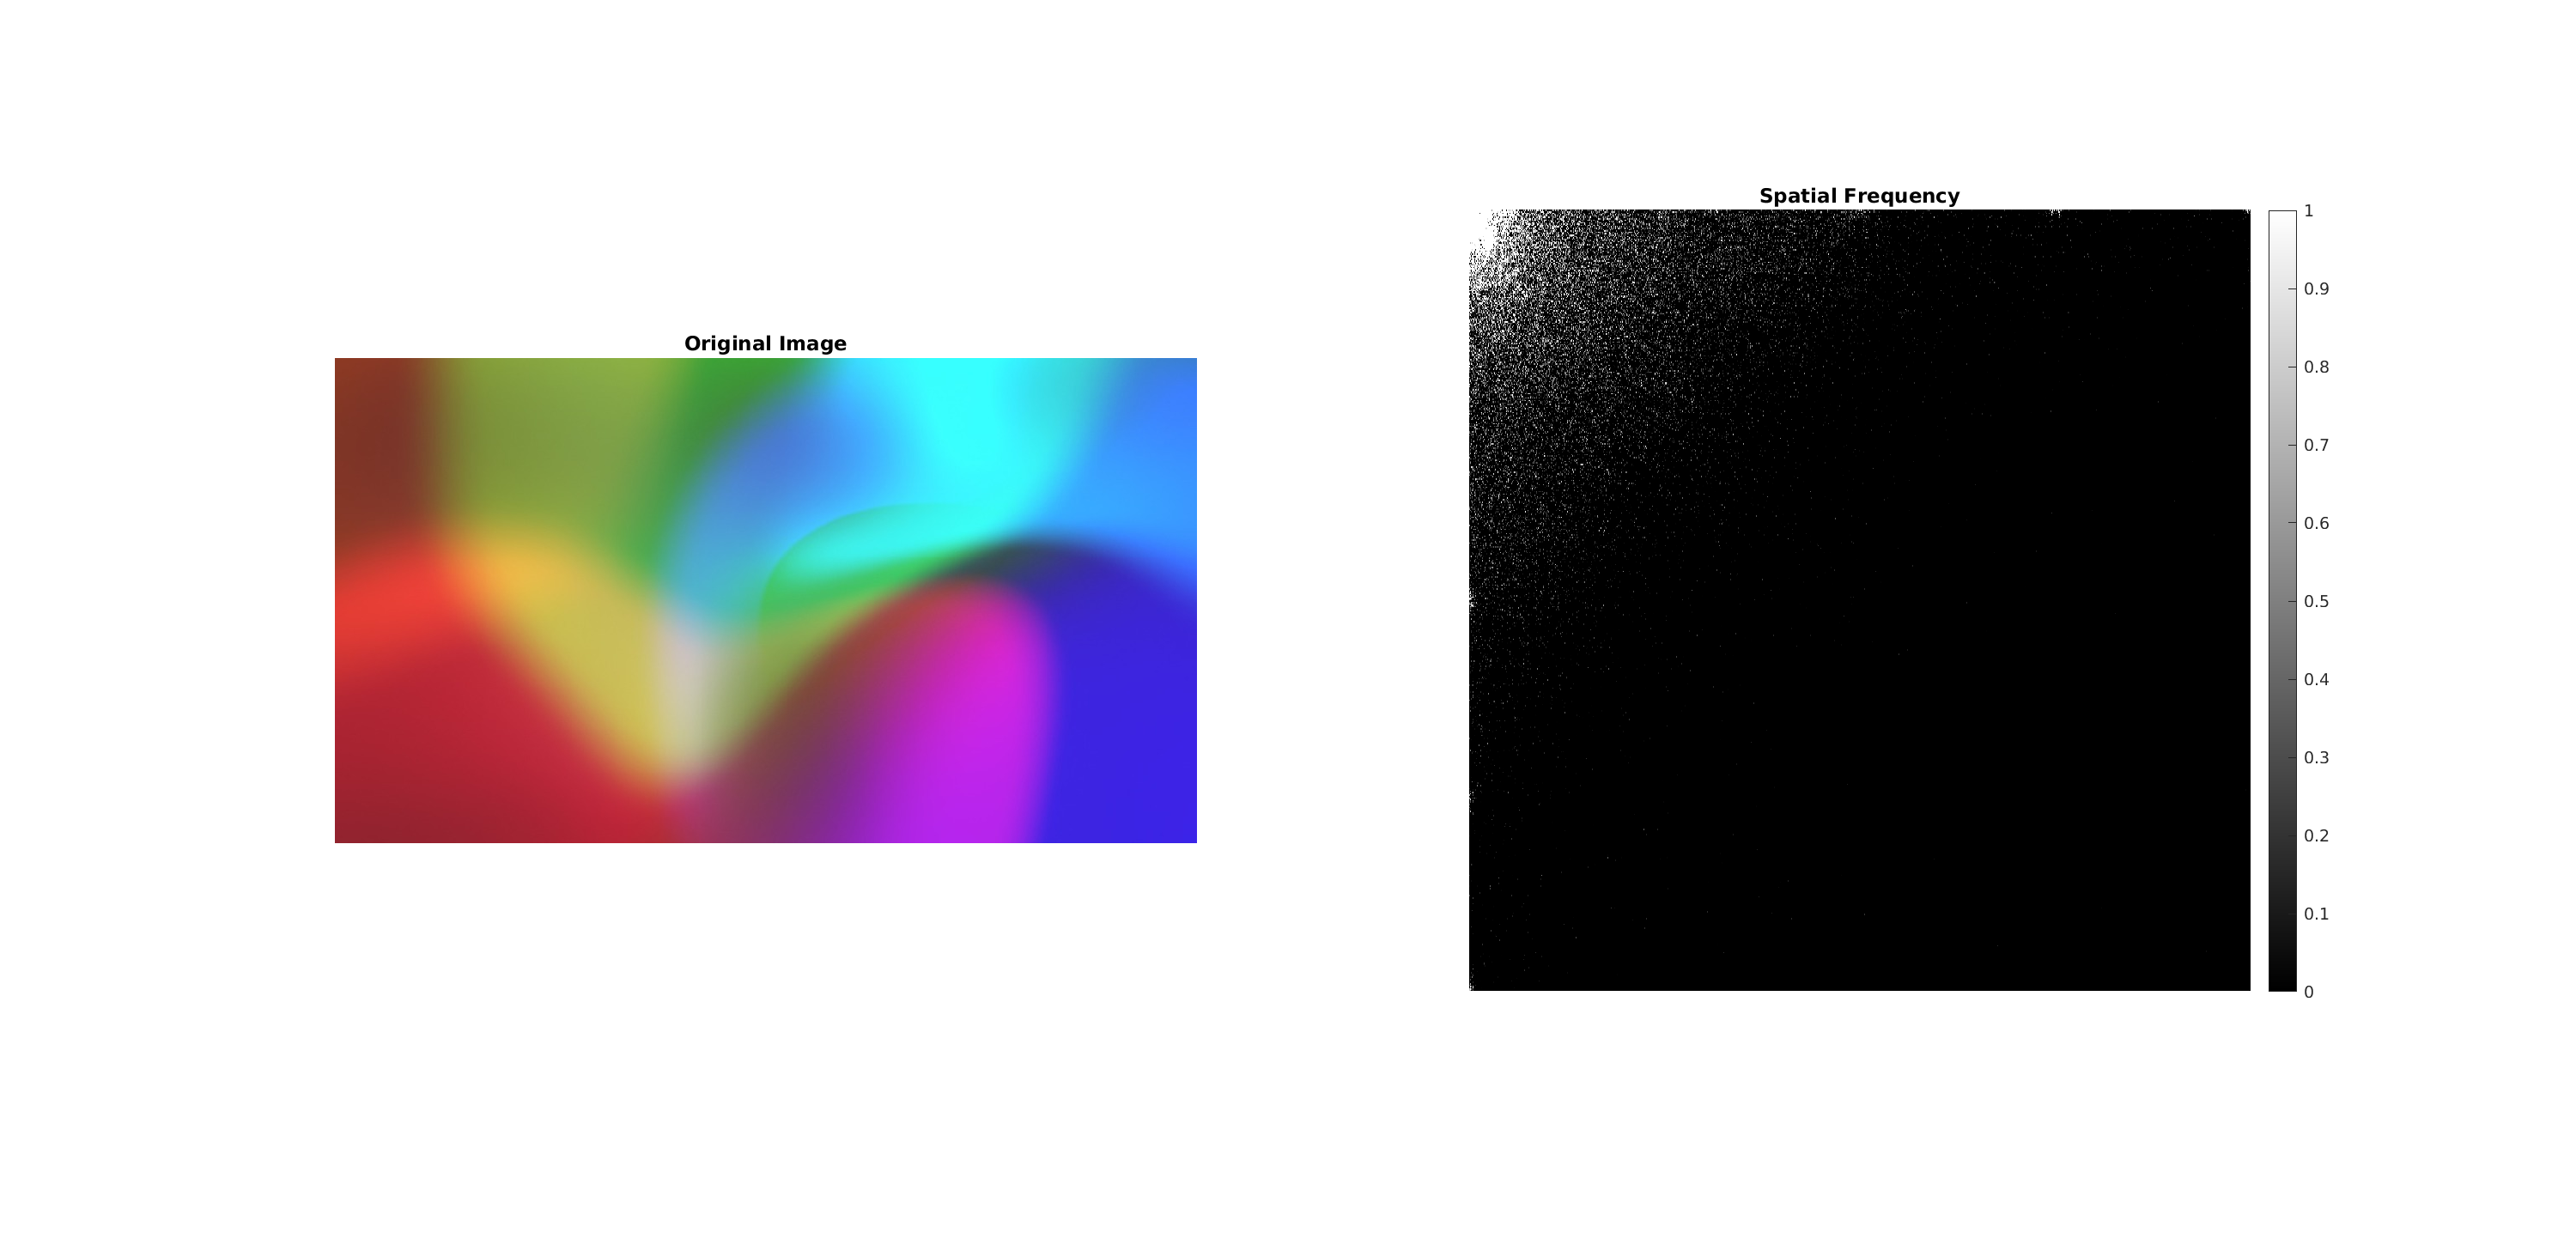
\includegraphics[width=\textwidth]
        {images/lsbrgb/dct/blurry_DCT.png}}
        \caption{\label{fig:lowfreq2} "Blurry": Low frequency image (left) and spatial frequency distribution (right)}.
      \end{figure}
      \begin{figure}[H]
        \center{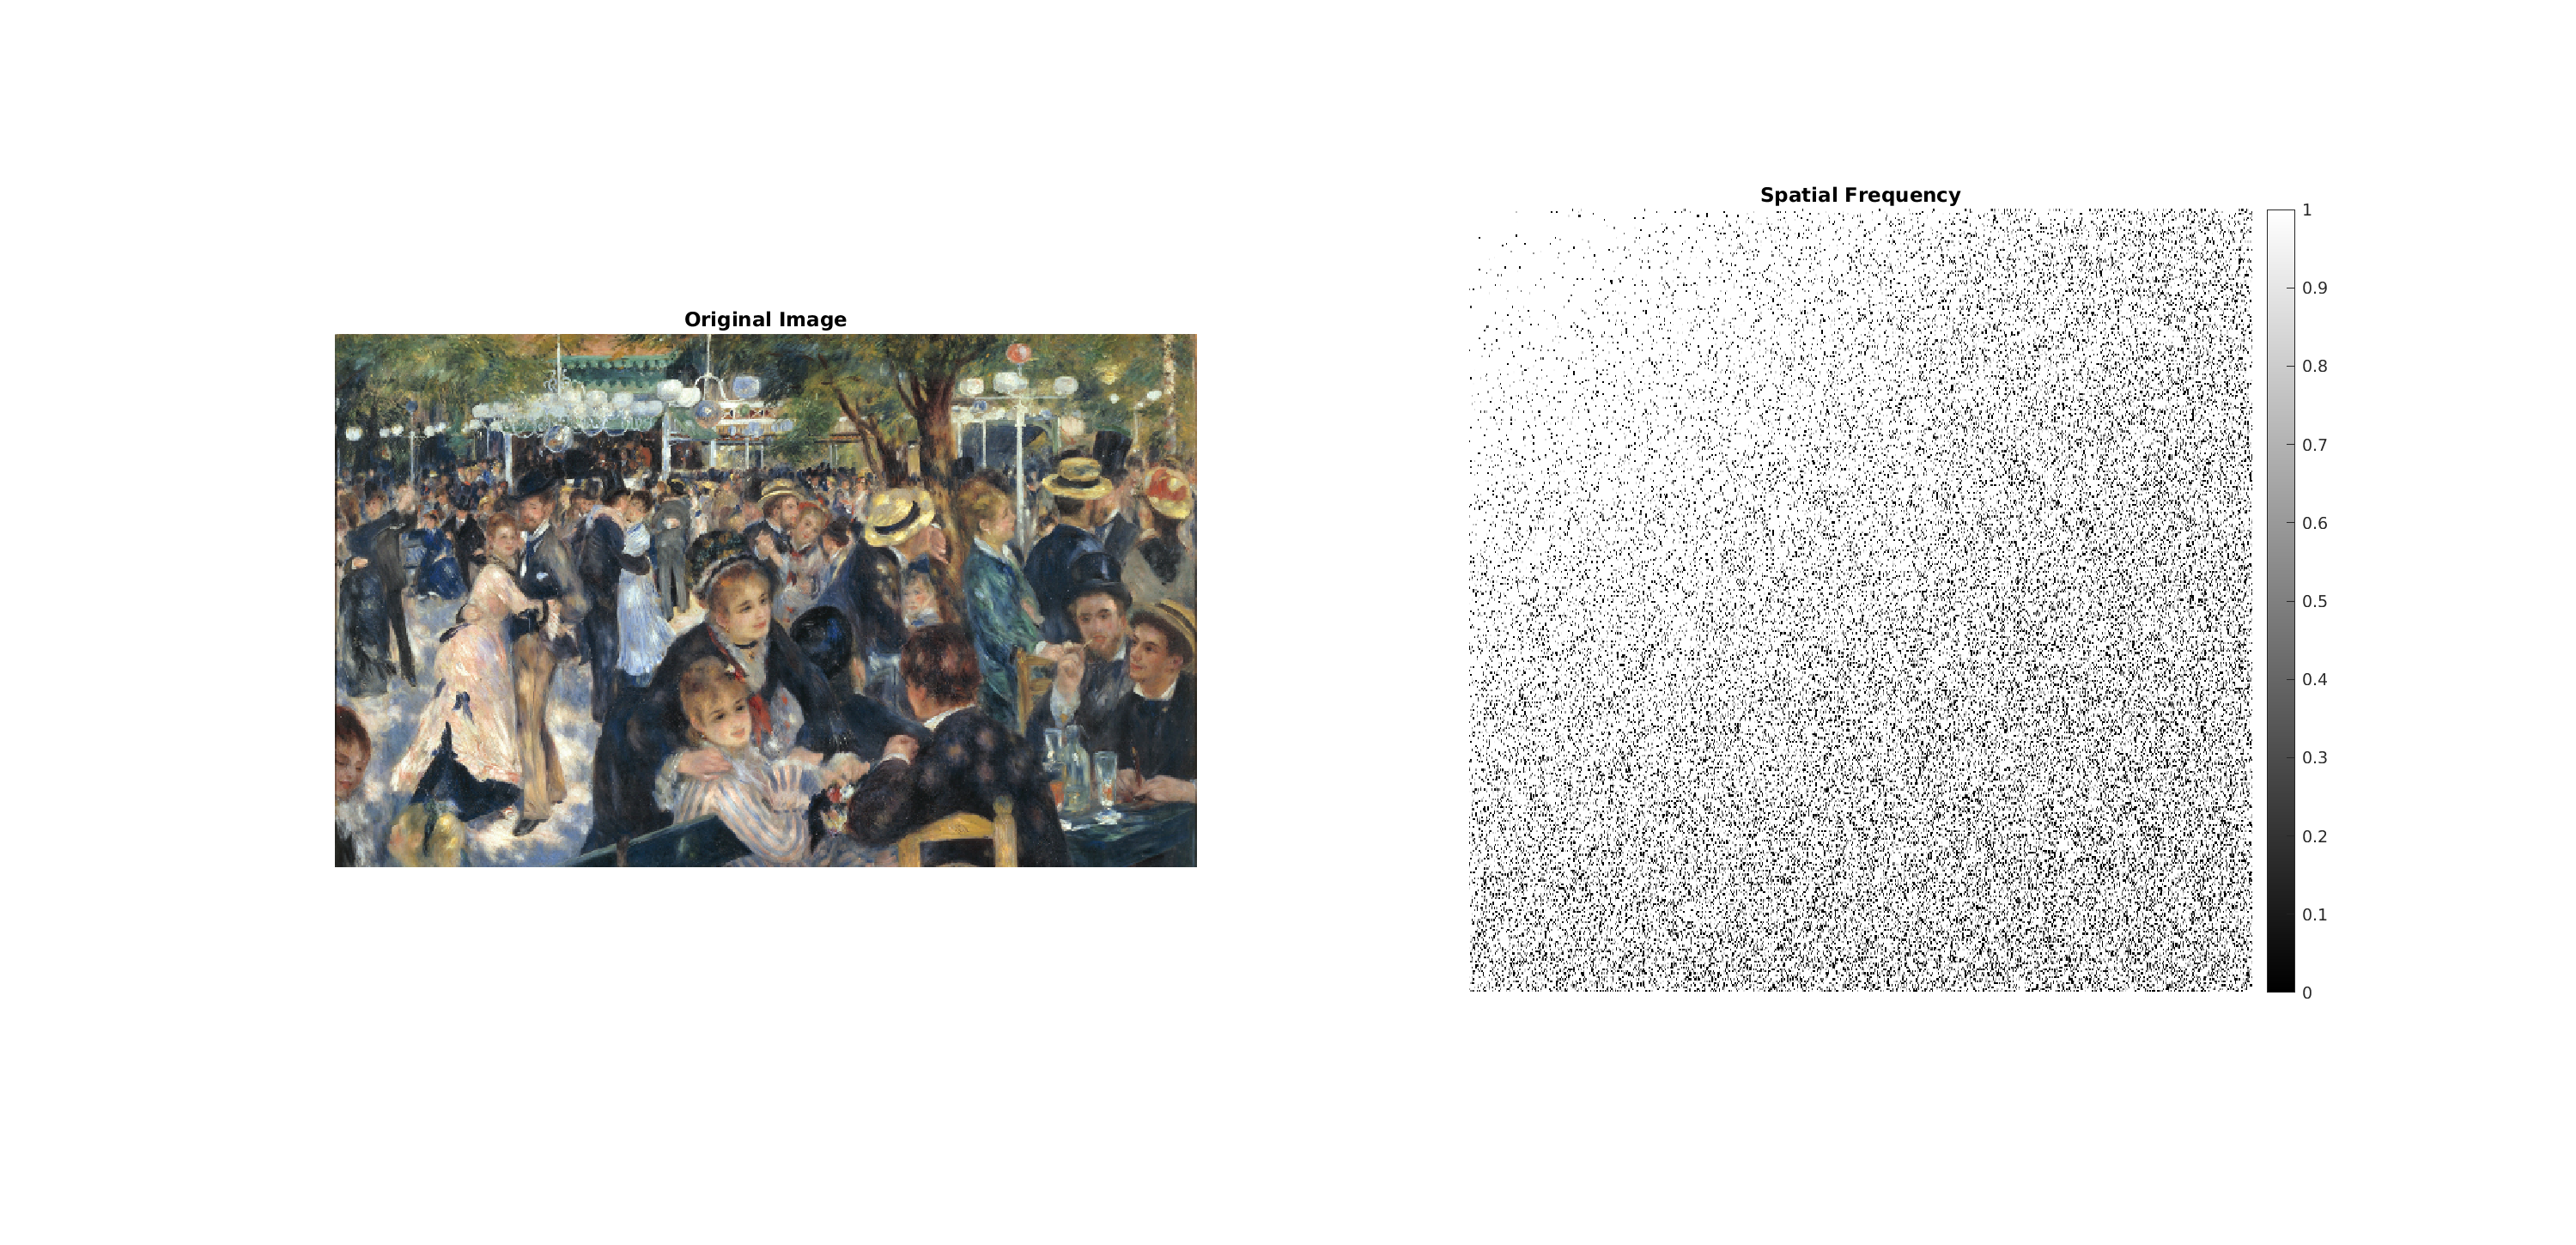
\includegraphics[width=\textwidth]
        {images/lsbrgb/dct/Galette_DCT.png}}
        \caption{\label{fig:highfreq2} "Galette": High frequency image (left) and spatial frequency distribution (right)}.
      \end{figure}      

	 Using the online image steganography tool, each of three images (Figure \ref{fig:highfreq} to \ref{fig:lowfreq}) were combined, using the first, second, and fourth lowest bit planes. The two high frequency images (Figure \ref{fig:highfreq} and Figure \ref{fig:highfreq2}) and the two low frequency images (Figures \ref{fig:lowfreq} and \ref{fig:lowfreq2}) were also merged.
	 
	For aim \ref{spatialeffectivenessaim}, spatial frequency could be deemed useful if there is found to be some correlation between the results and the spatial frequencies of the images. For aim \ref{stegaimcover}, the best cover file would be the one that after hiding have the least visible changes compared to the original. The same metric could be used for aim \ref{stegaimhidden}. The cover image with another hidden would first be compared to the original image, and then to the hidden image. If artefacts can be spotted when compared with the original, then the cover image offers very weak protection, but if it can only be noticed when the hidden image is also shown, then the cover image offers some protection. If neither, then the cover image is very effective.
      
\subsection{Experimental Trials}

The resuls are shown in the style of a Cayley table, where the horizontal headers correspond to the cover image used, and the vertical headers correspond to the image that was hidden. A score of 1 to 10 is used for each combination, where 1 shows clearly the hidden image, and 10 is indecernible from the original cover image. An asterisk is used where no data was recorded.

\subsubsection{LSB1}

\begin{center}
\begin{tabularx}{\columnwidth}{|X|X|X|X|}
  \hline
    \backslashbox{Hidden}{Cover} & Colourful & Viaduct & Sky \\
  \hline
    Colourful & *  & 10  & 7   \\  \hline

    Viaduct   & 10  & * & 6   \\  \hline

    Sky       & 10  & 10  & *    \\  \hline

    Blurry    & * & * & 10   \\  \hline

    Galette   & 10  & * & * \\
  \hline
  \end{tabularx}
\end{center}

\subsubsection{LSB2}

\begin{center}
\begin{tabularx}{\columnwidth}{|X|X|X|X|}
  \hline
    \backslashbox{Hidden}{Cover} & Colourful & Viaduct & Sky \\
  \hline
    Colourful & *  & 8  & 4   \\  \hline

    Viaduct   & 10 & *  & 3   \\  \hline

    Sky       & 10 & 9  & *    \\  \hline

    Blurry    & *  & *  & 9   \\  \hline

    Galette   & 10 & *  & * \\
  \hline
  \end{tabularx}
\end{center}

\subsubsection{LSB4}

\begin{center}
\begin{tabularx}{\columnwidth}{|X|X|X|X|}
  \hline
    \backslashbox{Hidden}{Cover} & Colourful & Viaduct & Sky \\
  \hline
    Colourful & *  & 3  & 2   \\  \hline

    Viaduct   & 7  & *  & 2   \\  \hline

    Sky       & 10 & 5  & *    \\  \hline

    Blurry    & *  & *  & 4   \\  \hline

    Galette   & 8  & *  & * \\
  \hline
  \end{tabularx}
\end{center}

\subsection{Outcomes}

For LSB1, the following notes were taken:

\begin{itemize}
	\item Top portion of Sky image gained unnatrual textures when colourful was the hidden image.
	\item Vertical columns in viaduct were faintly visible when hidden under sky image (Figure \ref{fig:skyviaductlsb1}).
\end{itemize}

\begin{figure}[htb]
    \centering
    \subfloat[Original Sky Image]{{\includegraphics[width=5cm]{"images/lsbrgb/sky_lowfreq"} }}
    \qquad
    \subfloat[Viaduct hidden in Sky Image.]{{\includegraphics[width=5cm]{"images/lsbrgb/lsb1/"lsb1_sky_viaduct"} }}
    \caption{Sky before and after viaduct was hidden using first least significant bit plane.}
    \label{fig:skyviaductlsb1}%
\end{figure}

For LSB2:

\begin{itemize}
	\item Viaduct image with colourful image hidden showed circle bright spots in sky. Colour transitions became more sudden (posterization).
	\item Viaudct with sky hidden also suffered from posterization
	\item Sky with viaduct and colourful hidden begins to clearly show shapes in hidden images.
\end{itemize}

And finally for LSB3:

\begin{itemize}
	\item Colourful with viaduct hidden only hints at hidden image in low frequency section (dark wall background).
	\item Colourful image with Galette appears brighter, slight texture in low frequency regions. 
	\item Viaduct with colourful definitely affected by posterization (Figure \ref{fig:viaductcolourlsb4}). Shows some textures from Colourful image in top portion, though rest is fairly unaffected.
\end{itemize}

\begin{figure}[htb]
    \centering
    \subfloat[Original Viaduct Image]{{\includegraphics[width=5cm]{"images/lsbrgb/viaduct_medfreq"} }}
    \qquad
    \subfloat[Viaduct image with Colourful image hidden.]{{\includegraphics[width=5cm]{"images/lsbrgb/lsb4/"lsb4_viaduct_colourful"} }}
    \caption{Viaduct before and after having Colourful hidden within using four least significant bit planes.}
    \label{fig:viaductcolourlsb4}%
\end{figure}

The results in regard to the aims of the experiment are:
\begin{enumerate}
	\item  Since higher spatial frequencies make artifacts harder to notice in an image, spatial frequency could be useful to determine if an image is effective as a cover image.
	\item  A highly detailed image is best suited to the purpose of cover image. 
	\item  Hiding a low frequency image in a high frequency cover image provides the most concealement
\end{enumerate}

\subsection{Discussion}

From the results, the colourful high frequency image showed the least distortion when used as a cover image. Only areas of less detail (blocks of solid colour) would show hints of the images underneath. The effectiveness of the less detailed image (sky) as a cover image drops sharply as the number of least significant bits used increases, even when being used to camoflauge an image with similar spatial frequencies. From the results, it appears likely that a "white noise" image like television static would be most effective as a cover image.

The experiment could be improved by using a more standardised scoring method, such as the single stimulus continuous quality evaluation (SSCQE) \cite{imagescore}, as well as using more participants.

\section{PSNR as a Metric} \label{psnrmetric}

\subsection{Introduction}

Often the peak signal-to-noise ratio (PSNR) is used as a metric of image quality during compression. It can also be used to quantify the difference between two images \cite{psnr}. The higher the value of PSNR for the stego image, the more similar it is to the original cover image, which suggests that humans will not perceive that any image is hidden. PSNR is used for this purpose very often as it is fast to compute and trivial to implement \cite{5586786}. However, using the literal difference between pixels values has been argued to be ineffective, since steganography is most effective when the two images are perceptually similiar rather than similar at the byte level (which PSNR evaluates).  

\subsection{Aims}

The aim of this experiment is:
\begin{enumerate}
	\item To determine the usefulness of PSNR as metric when choosing a cover image for LSB2 steganography.
\end{enumerate}

\subsection{Methods}
      
A Matlab script (\textit{calcPSNR.m}) was used to calculate the value of PSNR between the luminance channels of two images. The luminance channel was used as this is the aspect of images that the human eye is most sensitive to \cite{Thijssen1971}. This involves converting both images to YCbCr, and calculating the peak signal-to-noise ratio of the luminance (Y) channel of both images using 

\begin{equation}
	\textrm{PSNR} = 10 \log_{10} \Big( {\frac{\textrm{peakval}^2}{\textrm{MSE}}} \Big)
\end{equation}

where $\textrm{peakval}$ is the max value of the channel ($255$ for an 8-bit luminance channel) and $\textrm{MSE}$ is the mean square error \cite{matlabpsnr}.

Using the same images from experiment 1, the value of PSNR was calculated between the stego image and the cover image. If a low PSNR value corresponds to an ineffective stego image when plotted, this correlation can be confirmed.
      
\subsection{Experimental Trials}

The results are plotted in figure \ref{fig:psnrplot}. The script \textit{psnrForAllLSB.m} was run for each original image to produce \textit{test.csv}, to which the perceptual scores were then added manually. 

      \begin{figure}[H]
        \center{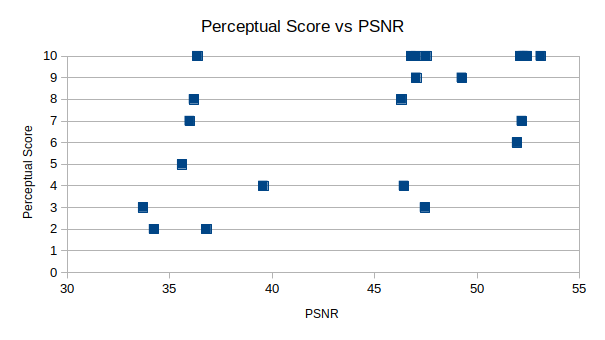
\includegraphics[width=\textwidth]
        {images/psnr/psnr}}
        \caption{\label{fig:psnrplot} Perceptual scores from experiment 1 against PSNR values of cover image and the stego image.}
      \end{figure}

\subsection{Outcomes}

No clear correlation between peak signal-to-noise ratio and the perceptual quality score can be seen. 

\subsection{Discussion}

The experiment was carried out on very few images, and relies on the result of the previous experiment which already sufferred from few numbers and a non-standardized scoring method. Nonetheless, the results do not seem to suggest any correlation between PSNR and perceptual quality of the stego image, which agrees with other experiments \cite{5586786}. Having realised this, most literature on modern steganography favours the use of the structural similarity index (SSIM) as a metric for how similar two images are in terms of human perception \cite{ssim}.

\part{Penetration Testing}

The tools and processes described in Broad and Binder \cite{binder} were utilised for this part. 

\section{Reconnaissance}

The online tool DNSInspect provided a warning that all name servers for the site are located on a single C class network \cite{dnsinspect}. This is a possible single point of failure which can be mitigated by spreading the name servers both geologically and topologically. 

Whois shows that the domain name is assigned to two people in West Yorkshire (Alex Parker and Mark Ducadi), at the address Eukhost Ltd, 7 Commercial Street, Morley, West Yorkshire, LS27 8HX. This information can be incredibly useful for social engineering and other exploits, and is required by ICANN. However, many services provide protection for WhoIs information which will mask the data with generic or unrelated contact details \cite{whoisprotec}.

Saving an offline copy of the site and examining the source files using the command \url{wget -m -p -E -k -K -np -v http://cybertest.uk} allowed for further examination. A few commented out lines in the \url{cybertest.uk.html} document provided a link to a motivating cover of the Game of Thrones theme \cite{got}, as well as a test user account \url{testuser@cybertest.uk} with a possible password \url{test underscore user1}. This kind of problem can be avoided through a development cycle involving peer reviews. Once removed, the username and password would likely have to changed or removed from the system in order to avoid it being utilised by attackers in the future. Many Github repositories suffer from a similiar issue, where developers allow configuration files containing sensitive data such as passwords to be publicly available. 

Another commented out section of the HTML file points us to \url{http://cybertest.uk/Server/AboutUs.asp}. This is an Active Server Page file, which suggests that the ASP.NET framework has been used for developing the site. 

The site does not support HTTPS, which means all connections are insecure as communications are made in plain text. Checking network requests and responses made when loading the page in Chrome, we can see that an Apache server is used to serve the website (Figure \ref{fig:servername}). This can be hidden by configuring the servers signature. Knowledge of the server type can help narrow down which attack types to use, and so obscuring this information is crucial.

      \begin{figure}[H]
        \center{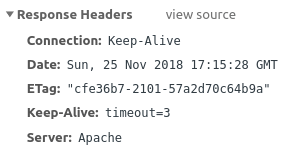
\includegraphics[width=6cm]
        {images/pentest/servername}}
        \caption{\label{fig:servername} Response headers on GET request to \textit{http://cybertest.uk/}}
      \end{figure}

\section{Scanning}

In order to assess the structure of the target network further, the command \url{nmap -sS -T4 http://cybertest.uk} was used (nmap with aggressive timing and stealth scan i.e. connections left open). A less agressive timing setting would be used if we wanted the scan to be harder to detect. The output (Figure \ref{fig:nmapoutput}) shows that several TCP ports are open. Specifially, the mail ports (pop3, smtps, pop3s, imap). There is also a mysql server running with the standard port open, which could potentially be accessed when coupled with the login details from earlier. Databases should almost never be accessible to the internet, as it is only necessary for the website server to communicate with the database, either through localhost or through a VPN. Since the database is open to the internet, brute forcing is an option. 

The UDP (\url{-sU}) scan was then tried, though this returned no results. From this we can conclude that it is possible that the ports are open, and/or filtered by a firewall. The ACK scan (-sA) was also carried out, which returned that all ports are unfiltered.

      \begin{figure}[H]
        \center{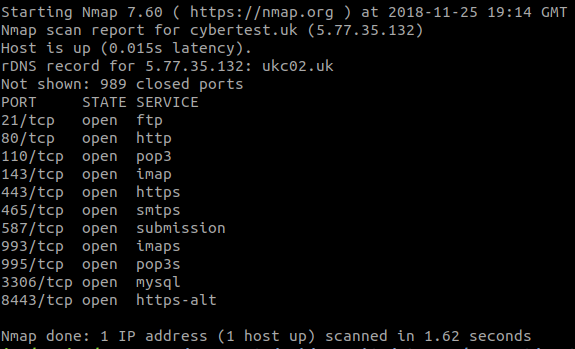
\includegraphics[width=\linewidth]
        {images/pentest/nmap}}
        \caption{\label{fig:nmapoutput} Response headers on GET request to \lstinline{http://cybertest.uk/}}
      \end{figure}
      
Port scans are difficult to protect against, and so it is best to reduce the number of attack vectors that they would present. Closing unecessary services such as HTTP on an HTTPS only web server and not running in X11 mode will reduce the number of vulnerabilities on a system. TCP wrappers can also be used to limit the amount of information available during a port scan, which will compare the requesting IP address to a list of allowed and unallowed IP addresses before determining if access to the service should be provided \cite{portprotec}. This mechanism also protects against IP spoofing, as a reverse DNS lookup will be used on the requesting IP address. 

Not all services can be protected this way (HTTP, SMTP), and if misconfigured can provide another attack vector to be exploited. Software such as PortSentry provides TCP wrappers and other methods of protection. For example, it will redirect packets from suspect IP addresses to a different or dead system in order to hide the system being attacked.
      
A Metasploit project was set up to target the IP address of $ 5.77.35.132 $ (\url{cybertest.uk}) in order to find out more information. After scanning, it was able to determine that MySQL 5.5.57 is being used, and that the server runs on Linux 2.6.X. The last boot time from the server was also shown as being a few day prior. An overview of the scans are shown in figure \ref{fig:overview}.

      \begin{figure}[H]
        \center{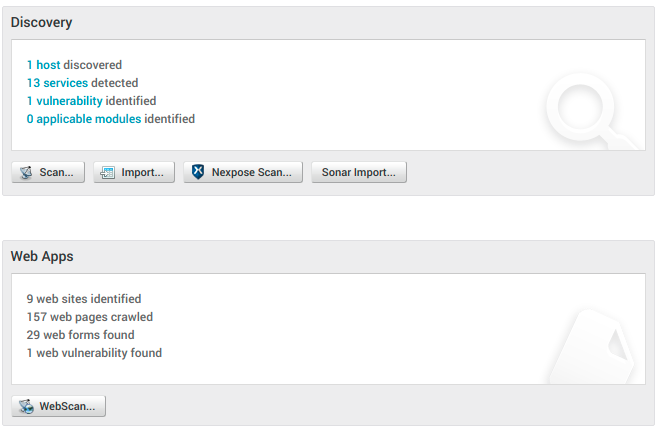
\includegraphics[width=\linewidth]
        {images/pentest/overview}}
        \caption{\label{fig:overview} Overview of Metasploit scan results.}
      \end{figure}
    
Two HTTPS ports were open. On port $8443$ the login page for UKC hosting could be found. This is the portal to managing the Plesk hosting service. After using the WebScan feature on Metasploit (WMAP), it was revealed that this login page did not have an anti CSRF token. In the OWASP "Cross-Site Request Forgery (CSRF) Prevention Cheat Sheet" \cite{owasp}, it specifically states that form tags using POST requests should be protected from CSRF vulnerabilties. The source for the login page at \url{https://ukc02.uk:8443/get_password.php} clearly features a form with method POST. This login page should preferably be hidden to the internet, and treated similiar to the database serivce, and an anti CSRF token should be used for the login form. 

The reason the CSRF token is necessary is due to the fact that once the user is authenticated to the service, the browser will automatically include credentials related to the site in all subsequent requests. This allows attackers to make requests as if they were the victim. The CSRF token is a piece of information that the attackers would not be able to access, therefore can be used to confirm that the request is from the expected user. Often the exploit uses the 'src' attribute of \textit{img} tags, as they would not be obvious to the user. 

\part*{Conclusion}

Both parts of this practical were enlightening and enjoyable. For part 1, reading about modern applications of steganography and its history was very interesting. Given more time, I would have like to have used the more reliable perceptual scoring methods referenced, as well as including more images in the dataset. 

For part 2, the recommended reading gave a clear step-by-step guide into the process of penetration testing. Understanding the output of the tools described and the way they work has definitely helped solidify my learning for the module. I would have liked to have taken it a step further and attempted the exploitation phase, but this would have been innappropriate. Instead, I plan on experimenting against my own web-based projects in order to improve them and my own abilties in security.

\part*{Appendix}

Matlab scripts, images, and result files from Part 1 can be found in directory named \textit{stego}. Scripts were run using Matlab version 2018b.

\bibliographystyle{unsrt}
\bibliography{mybib}

\end{document}
